\documentclass{article}
\usepackage[utf8]{inputenc}
\usepackage[brazil]{babel} % allow utf-8 input
\usepackage[T1]{fontenc}    % use 8-bit T1 fonts
\usepackage{hyperref}       % hyperlinks
\usepackage{url}            % simple URL typesetting
\usepackage{booktabs}       % professional-quality tables
\usepackage{amsfonts}       % blackboard math symbols
\usepackage{nicefrac}       % compact symbols for 1/2, etc.
\usepackage{microtype}      % microtypography
\usepackage{lipsum}
\usepackage{amsthm}
\usepackage{amsmath}
\usepackage{graphicx}
\usepackage{graphics}
\usepackage[square,numbers]{natbib}
\graphicspath{{Images/}}
\newcommand{\norm}[1]{\lVert#1\rVert}
\newcommand{\gama}{\gamma}
\newcommand{\Tau}{\Gamma}
\newcommand{\ues}{\{\emptyset\}}
\usepackage{ragged2e}
\pagestyle{plain}
\title{Trabalho Funções Hiperólicas}
\author{Paulo Henrique Baratella Mattos}
\date{10893124}

\begin{document}

\maketitle

\section{Comparação entre os Métodos}
Os testes foram feitos a partir das condições pedidas: $t = 17s, 0\leq  x\leq 25, h=0.05$ e $k = 0.8h$. A seguir segue alguns detalhes da realização das comparações:\\
A linha laranja ao fundo é a solução exata e as bolinhas representam a solução dos métodos.\\ 
Note que não há o método \textit{Esquema Central},já que, por não ser estável, não possibilita que seu gráfico seja renderizado pelo Octave.\\
O método \textit{Leapfrog} pede valores referentes à 2 partições de tempo anteriores da iteração atual. Como é somente dado o valor do momento $t=0$, e não encontrei uma maneira convencionada de resolver os valores do tempo $t=k$, tomei a liberdade de defini-los como os valores calculados pelo método \textit{Upwind}.


\begin{table}
    \centering
        \begin{tabular}{ccccc}
            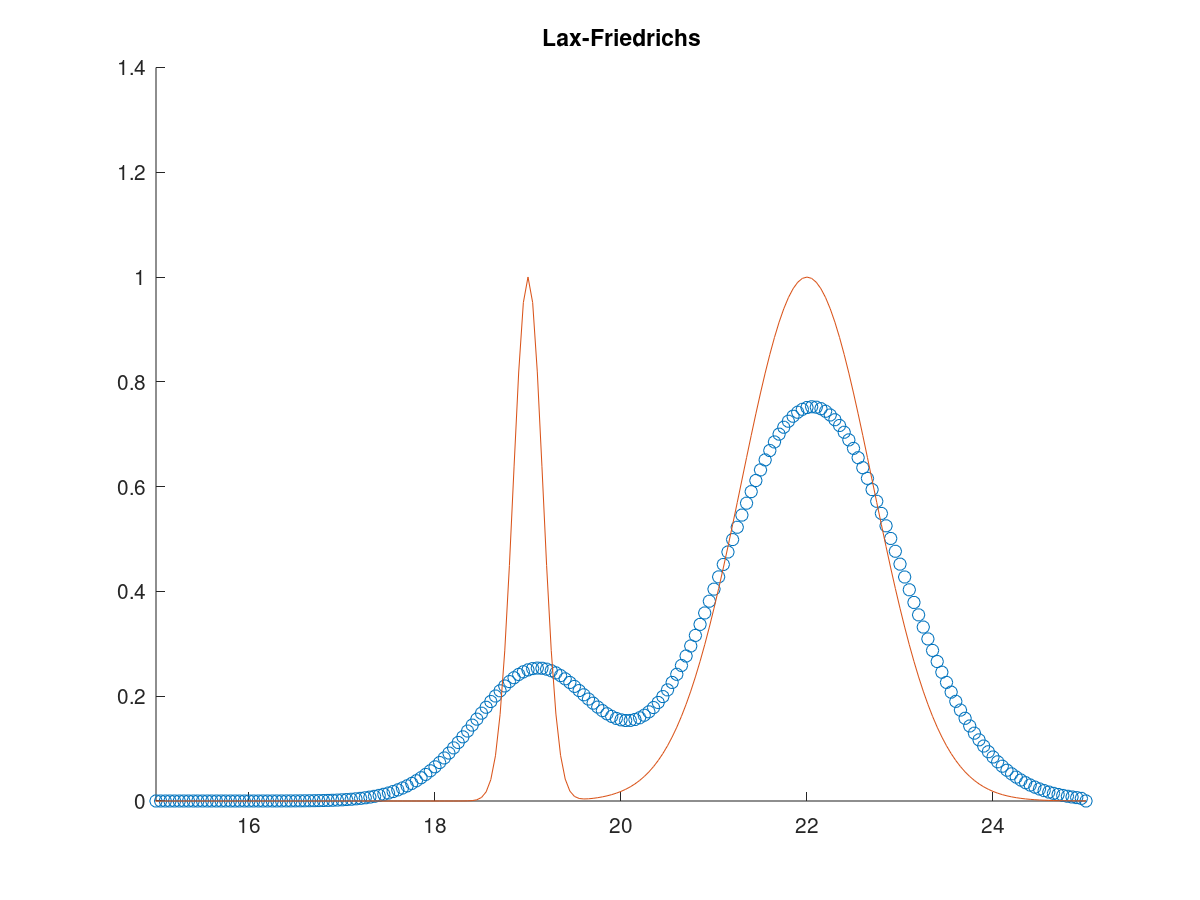
\includegraphics[scale = 0.17]{LF.png} & 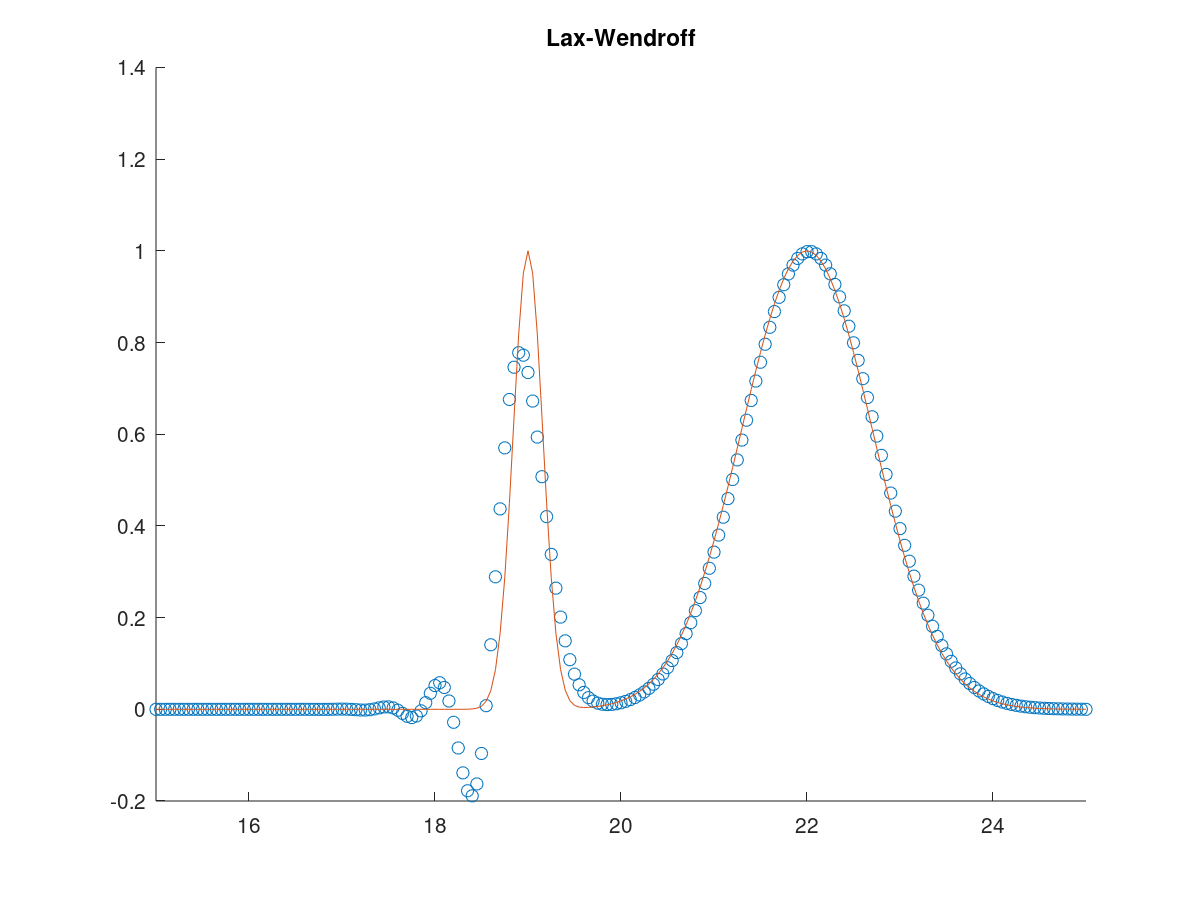
\includegraphics[scale = 0.17]{LW.png} \\
            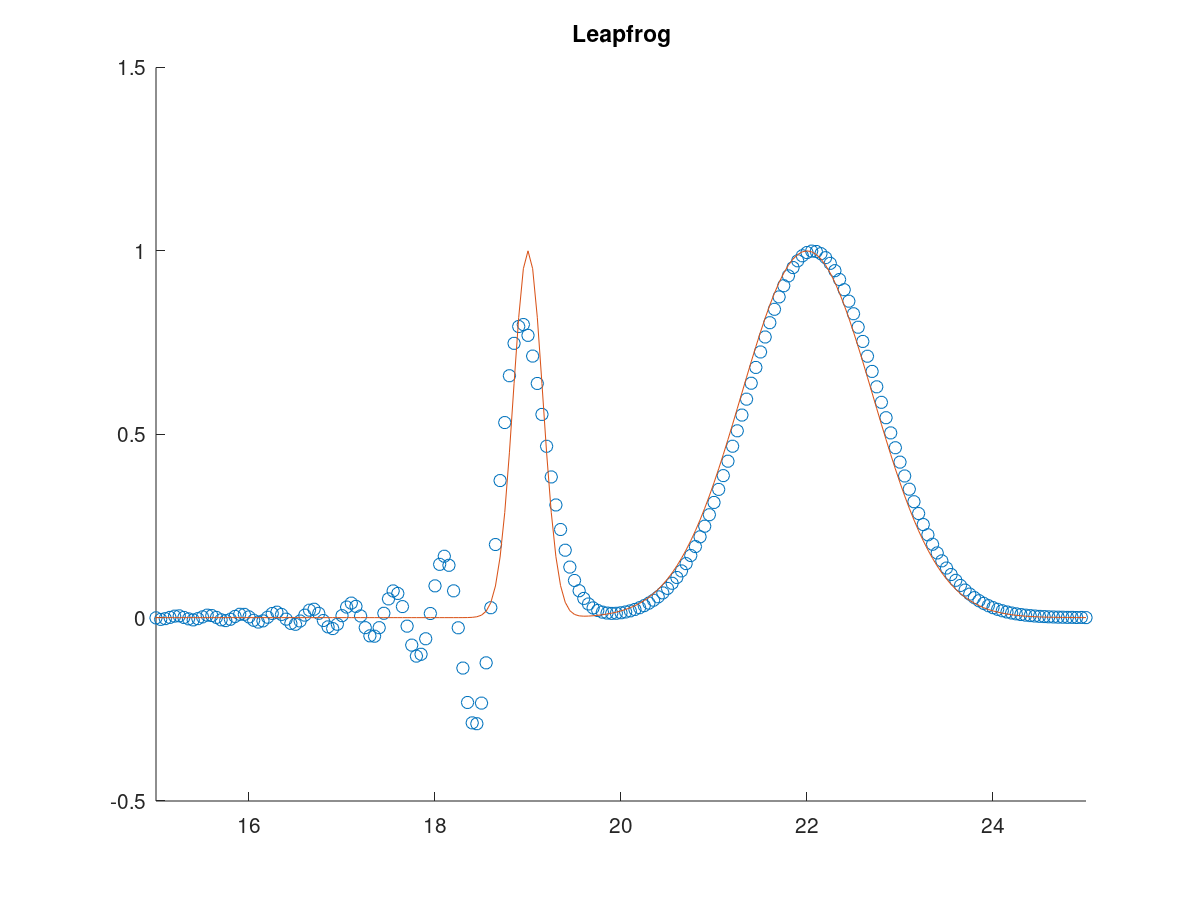
\includegraphics[scale = 0.17]{Leapfrog.png} & 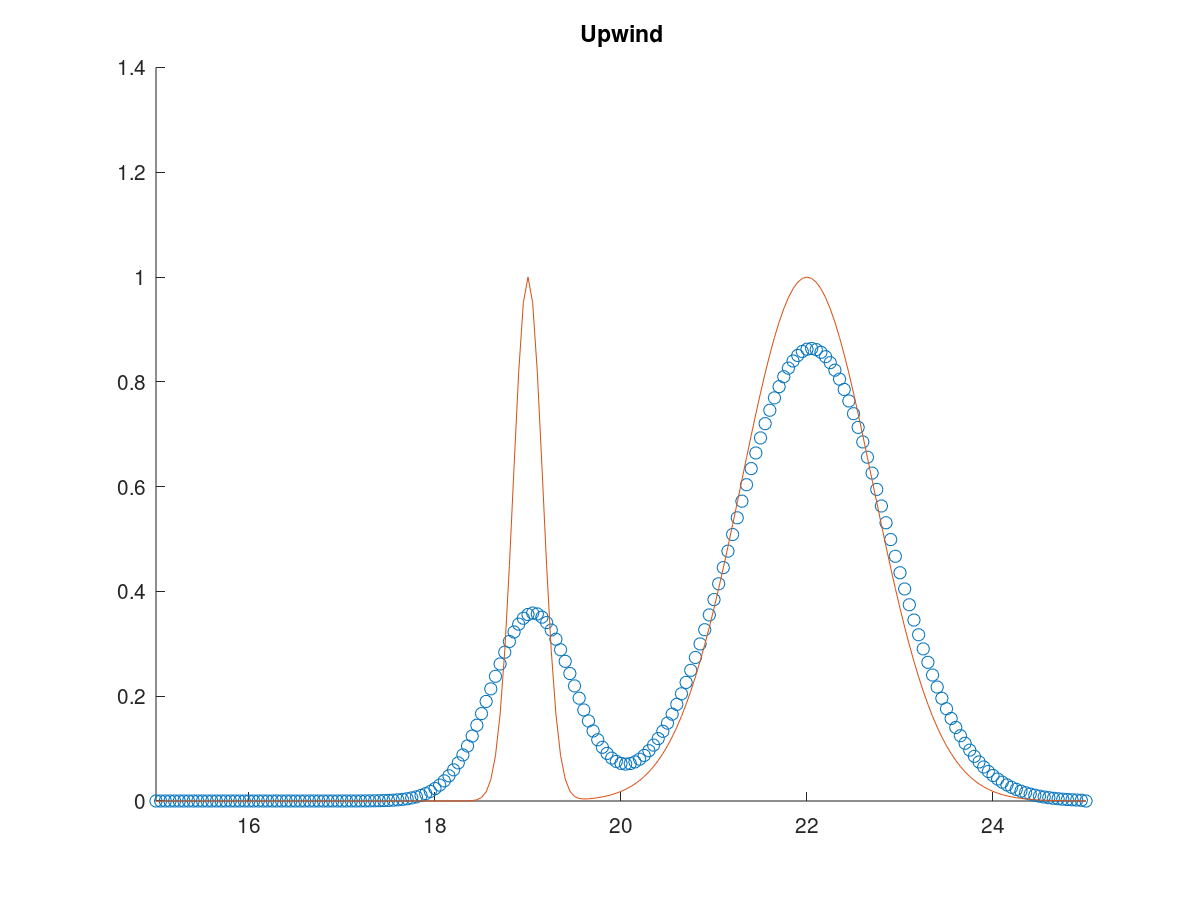
\includegraphics[scale = 0.17]{Upwind.png}
        \end{tabular}
    \label{tbl:table_of_figures}
\end{table}

O comportamento mostrado é muito similar ao mostrado no livro de Leveque.
\newpage
\section{Extensões Temporais}

Ao extender o domínio de cálculo de $t_f=17$ para $t_f=34$ ocorre como nas imagens acima.\\
Não há mais nenhuma onda, isso ocorre pois ,por $a>0$, a onda se \textit{move para a direita} e, por não haver limites na equação original, ela sai do escopo do nosso conjunto.\\

Note que todos obtiveram valores muito próximos do correto, com erro na casa de $10^{-11}$, com exceção do $Leapfrog$ que apresenta uma dispersão enorme no meio do conjunto. É mais uma dispersão do que um instabilidade, ja que se dá simetricamente nos valores corretos.


\begin{table}
    \centering
        \begin{tabular}{ccccc}
            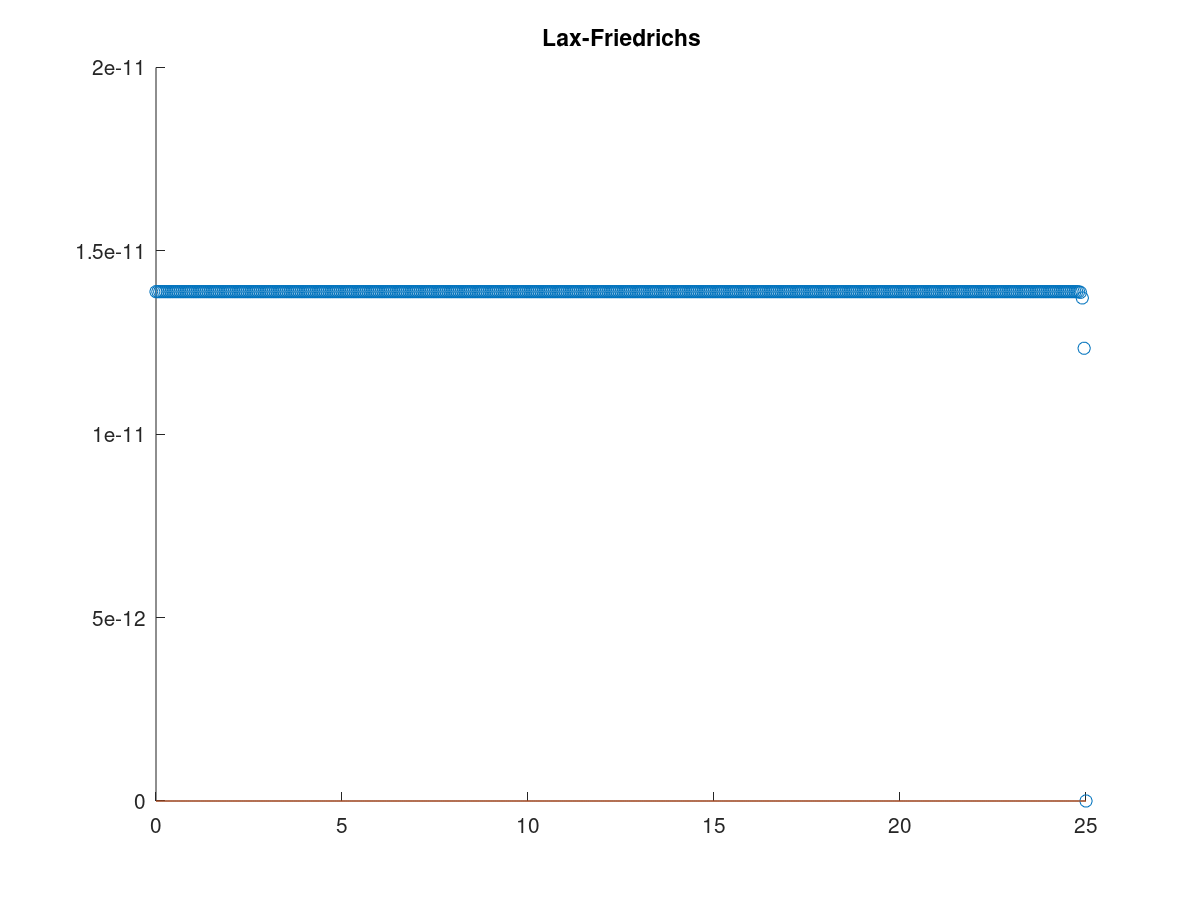
\includegraphics[scale = 0.15]{LF34.png} & 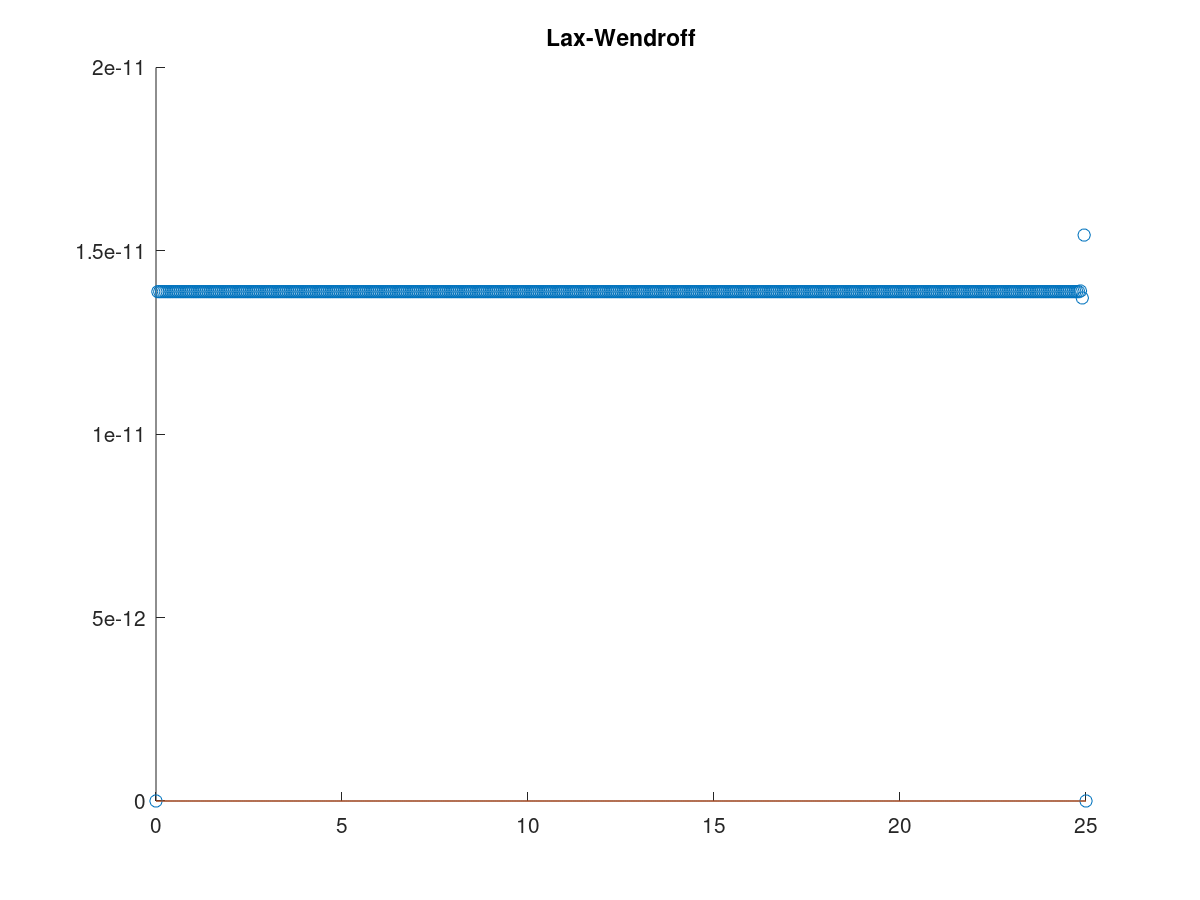
\includegraphics[scale = 0.15]{LW34.png} \\
            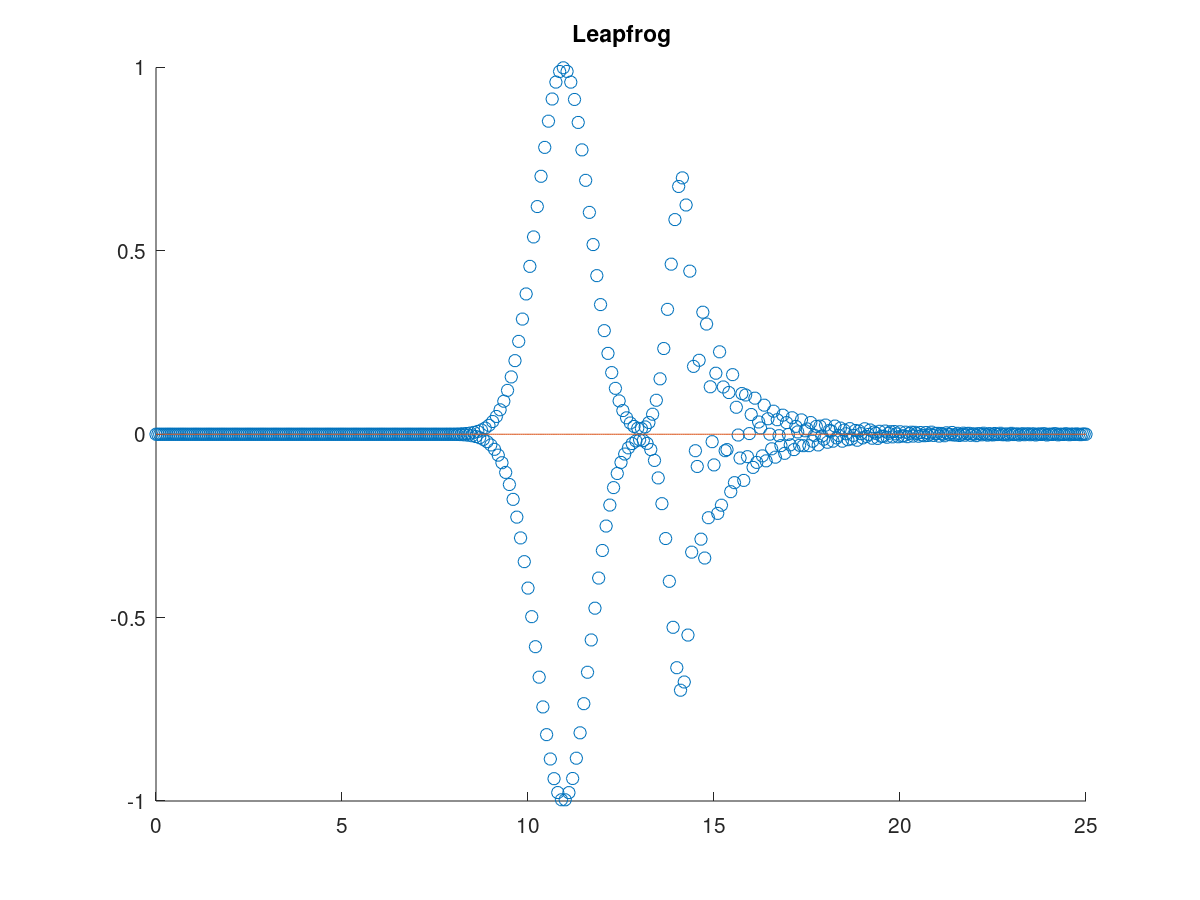
\includegraphics[scale = 0.15]{Leapfrog34.png} & 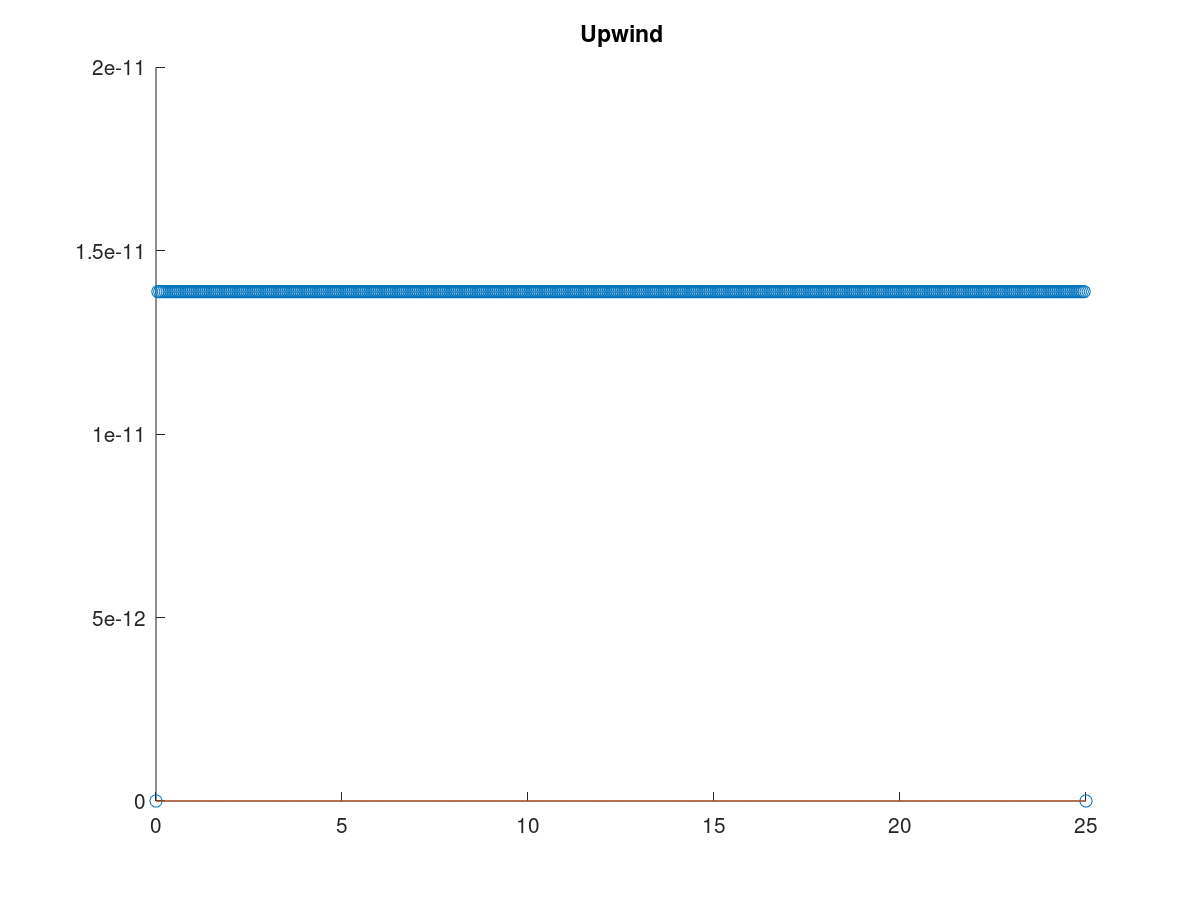
\includegraphics[scale = 0.15]{Upwind34.png}
        \end{tabular}
    \label{tbl:table_of_figures}
\end{table}


\newpage
\section{Refinamento de Malha}
Fiz 3 refinamentos (divisão por 2,4,8): $h = \{0.025,0.0125,0.00625\}$. Os outros valores são como o padrão da primeira parte, $t = 17$.


\subsection{Lax-Friedrichs}
\begin{table}[h]
    \centering
        \begin{tabular}{ccccc}
            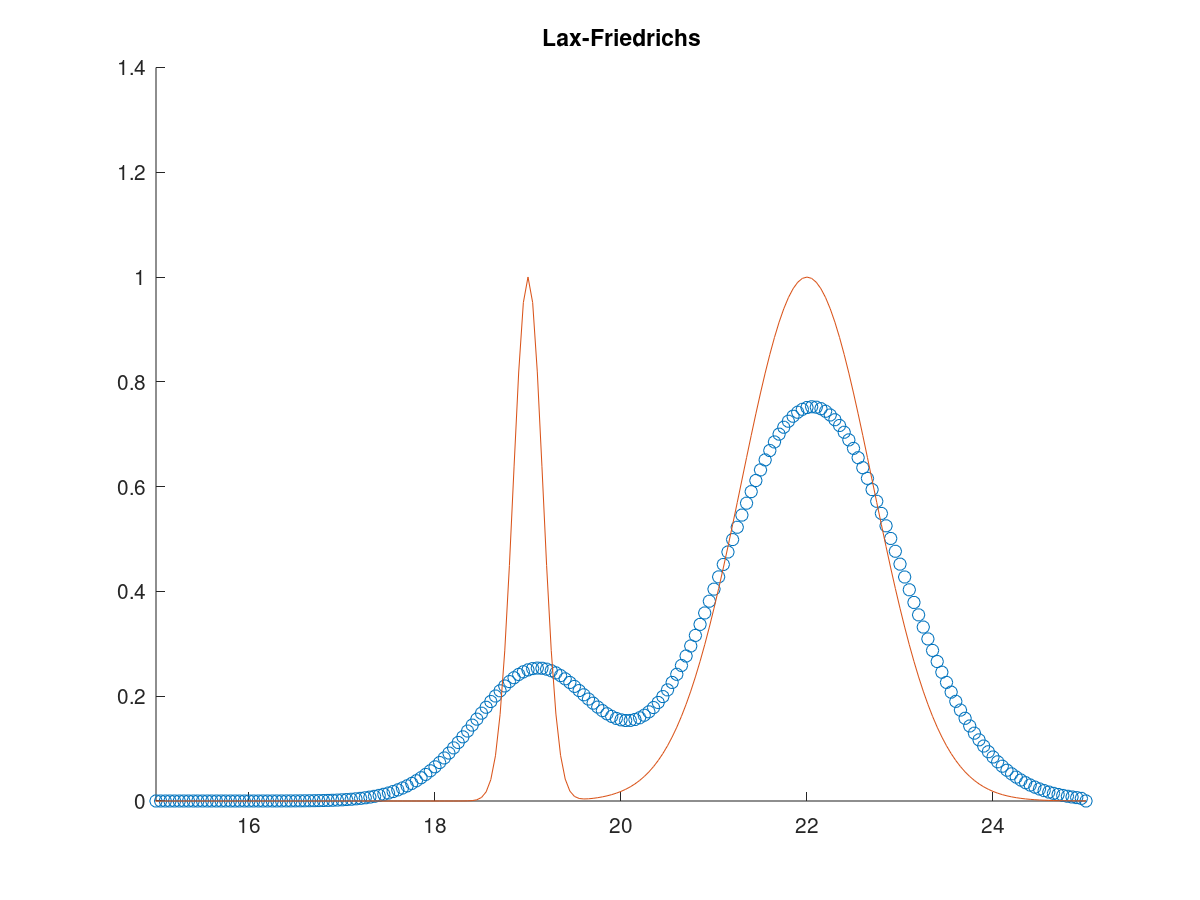
\includegraphics[scale = 0.17]{LF.png} & 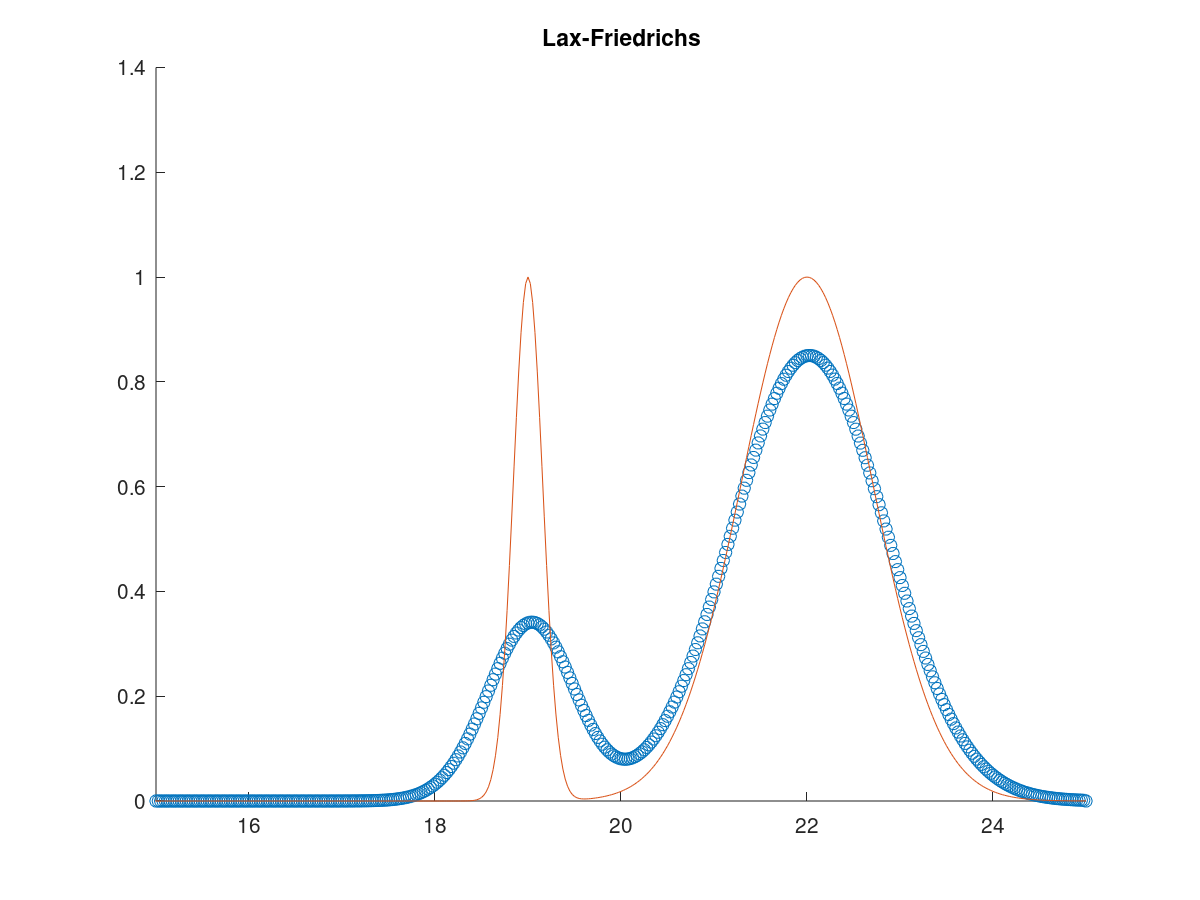
\includegraphics[scale = 0.17]{LF2.png} \\
            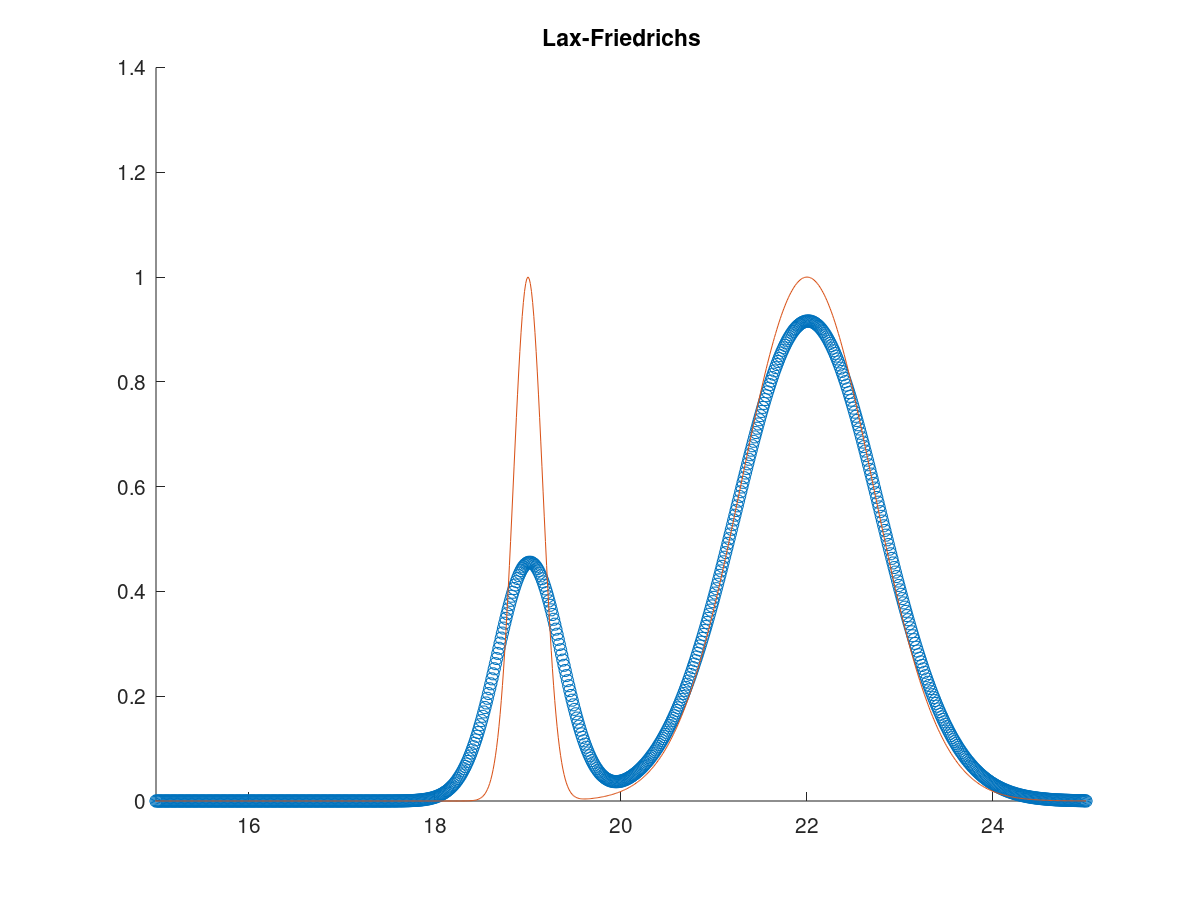
\includegraphics[scale = 0.17]{LF4.png} & 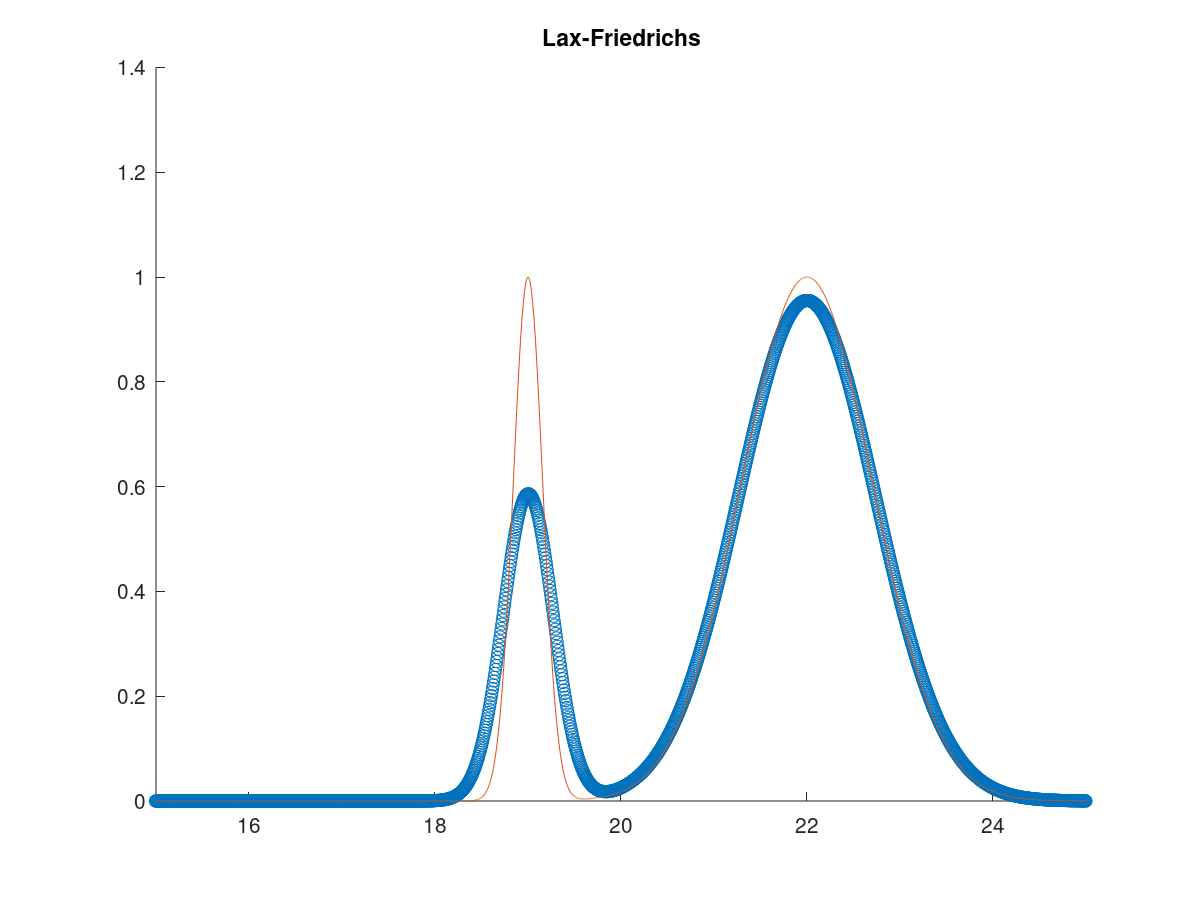
\includegraphics[scale = 0.17]{LF8.png}
        \end{tabular}
    \label{tbl:table_of_figures}
    \caption{Da esquerda para a direita são $h = 0.05, h = 0.025,h = 0.0125, h = 0.00625$}.
\end{table}
\newpage
\subsection{Upwind}
\begin{table}[h]
    \centering
        \begin{tabular}{ccccc}
            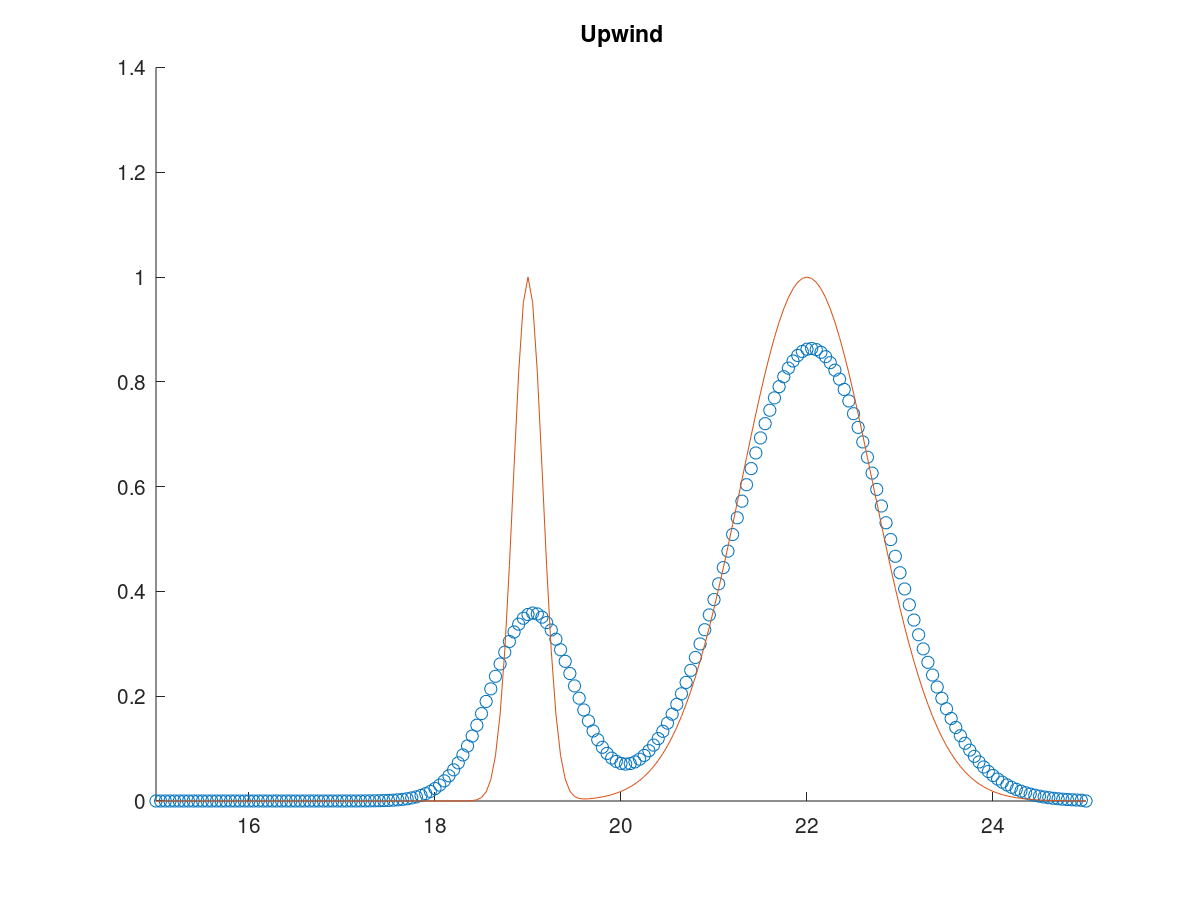
\includegraphics[scale = 0.17]{Upwind.png} & 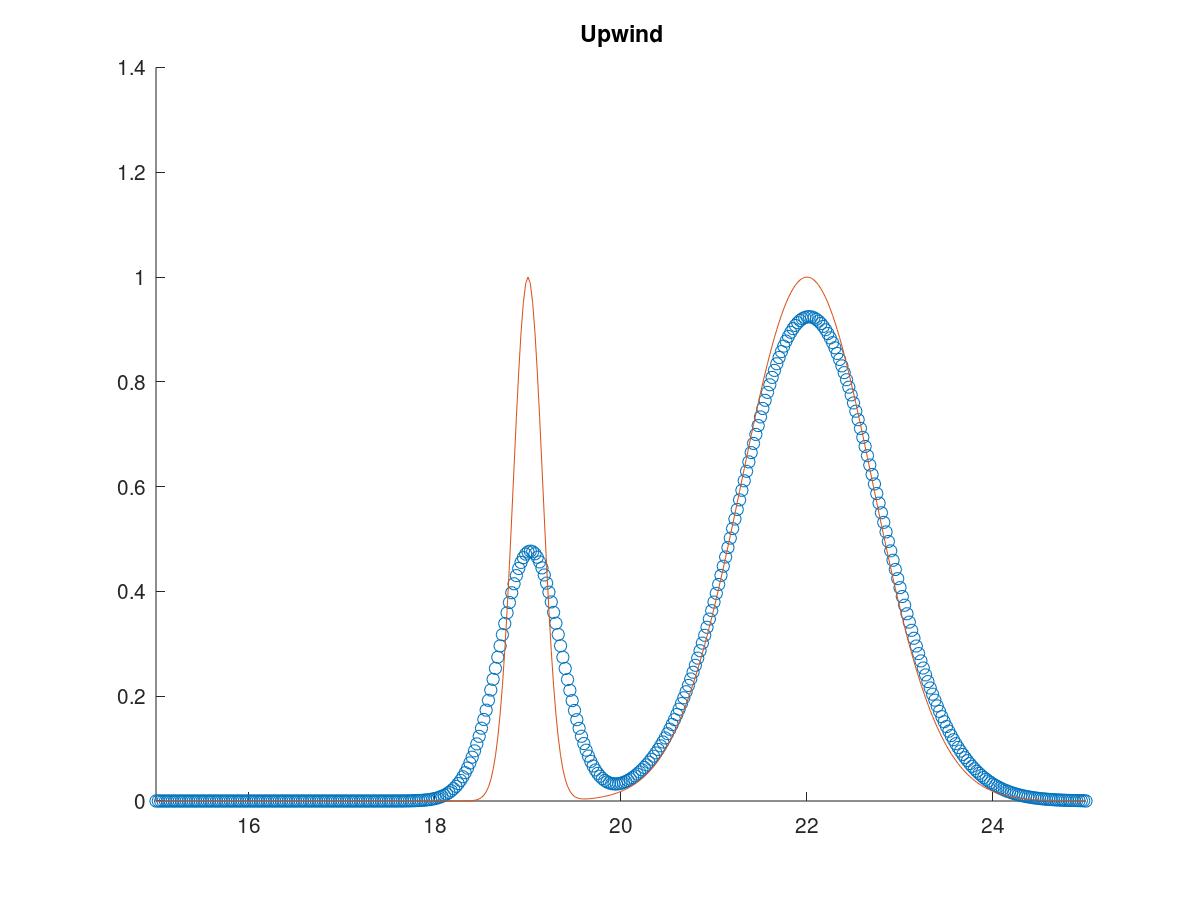
\includegraphics[scale = 0.17]{Upwind2.png} \\
            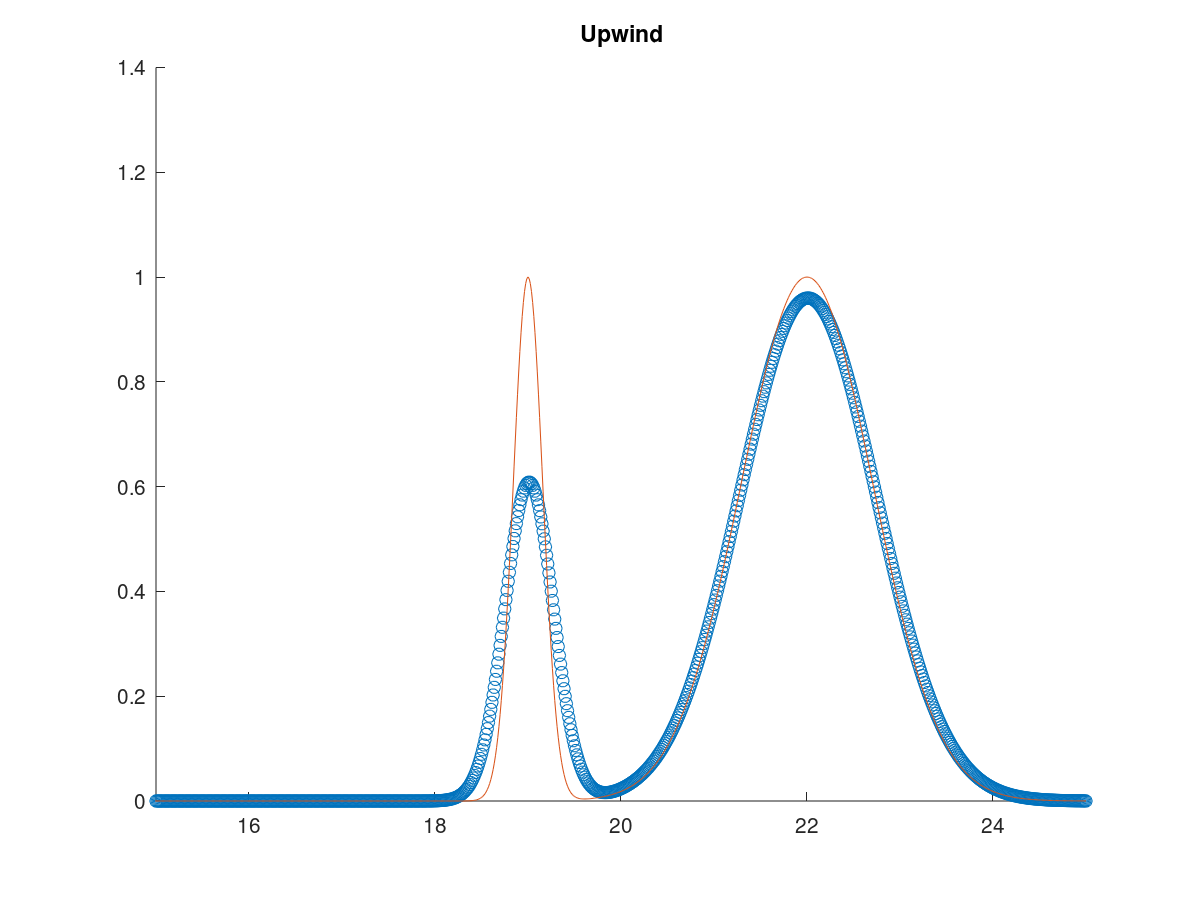
\includegraphics[scale = 0.17]{Upwind4.png} & 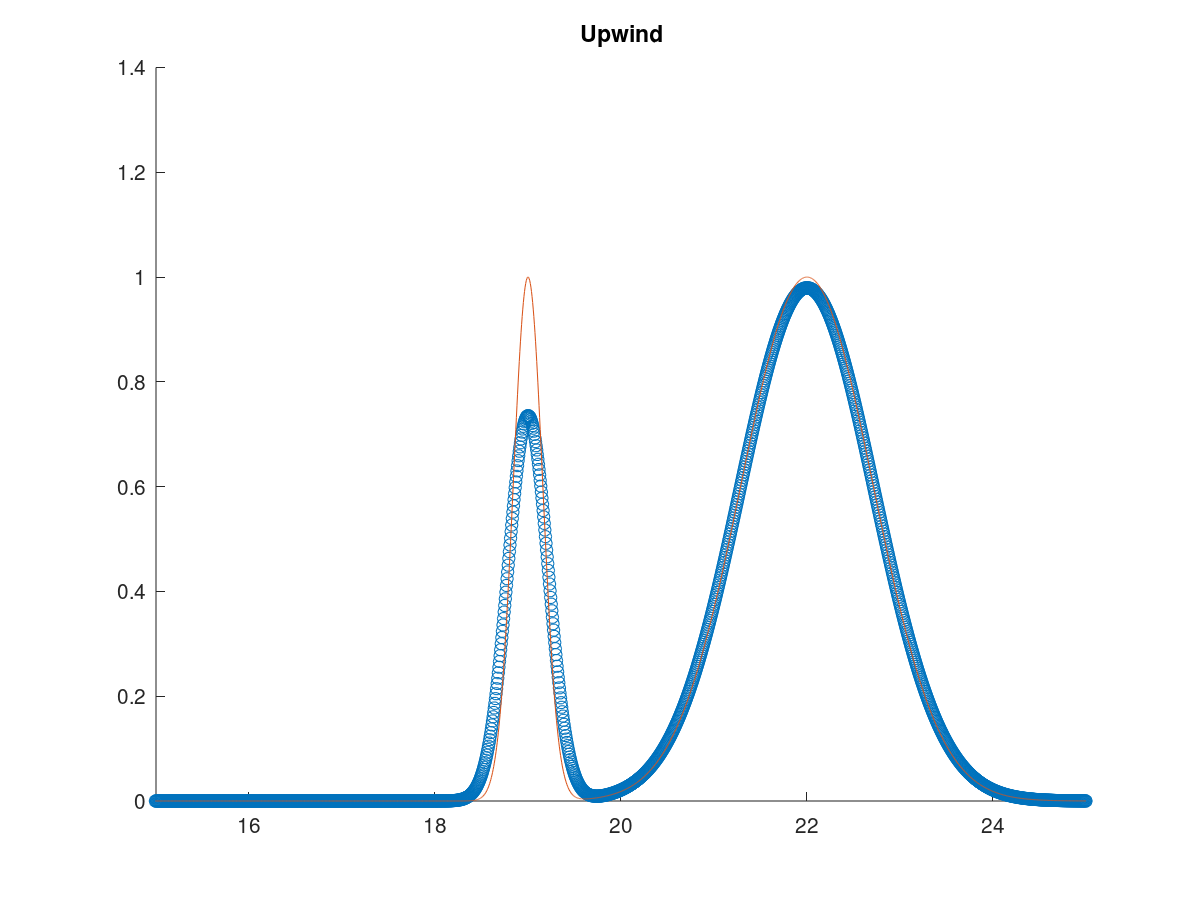
\includegraphics[scale = 0.17]{Upwind8.png}
        \end{tabular}
    \label{tbl:table_of_figures}
    \caption{Da esquerda para a direita são $h = 0.05, h = 0.025,h = 0.0125, h = 0.00625$}.
\end{table}
\newpage
\subsection{Leapfrog}
\begin{table}[h]
    \centering
        \begin{tabular}{ccccc}
            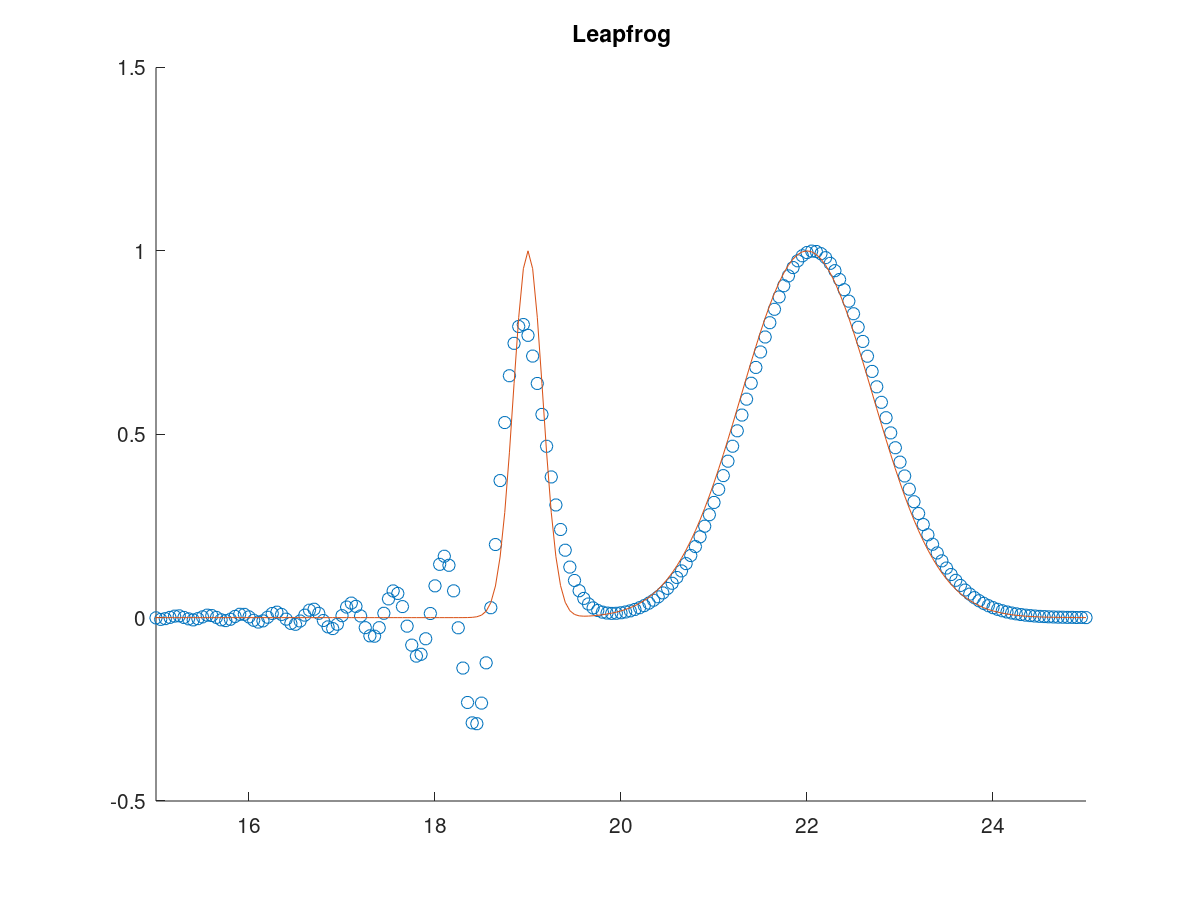
\includegraphics[scale = 0.17]{Leapfrog.png} & 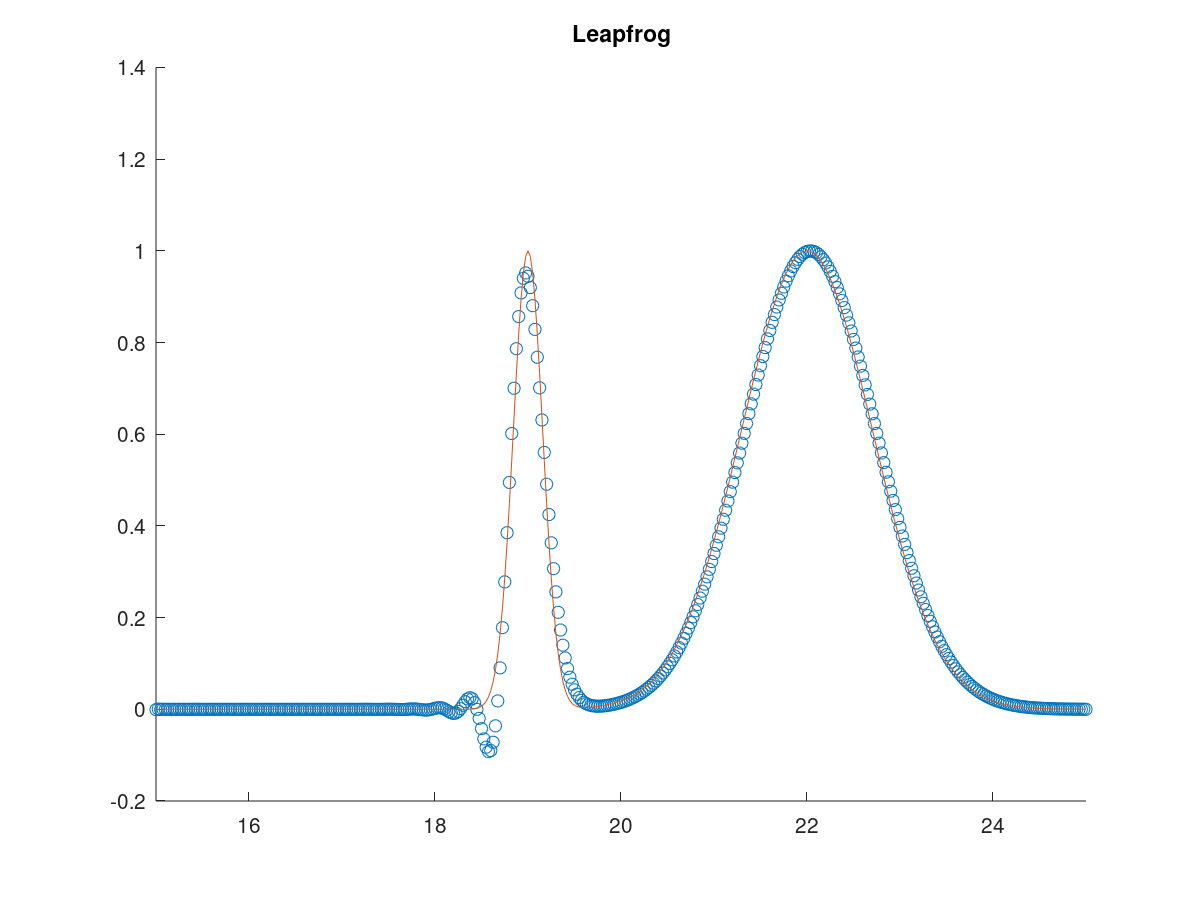
\includegraphics[scale = 0.17]{Leapfrog2.png} \\
            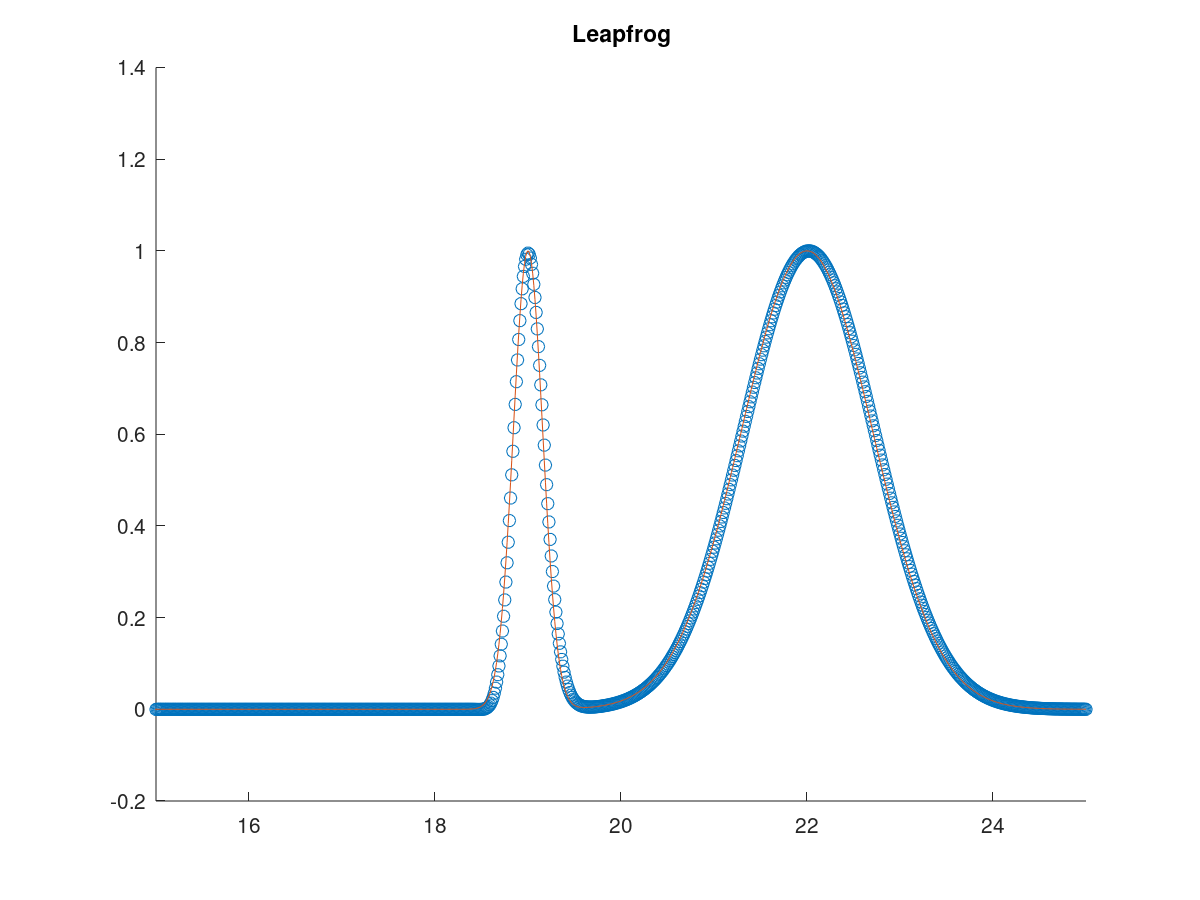
\includegraphics[scale = 0.17]{Leapfrog4.png} & 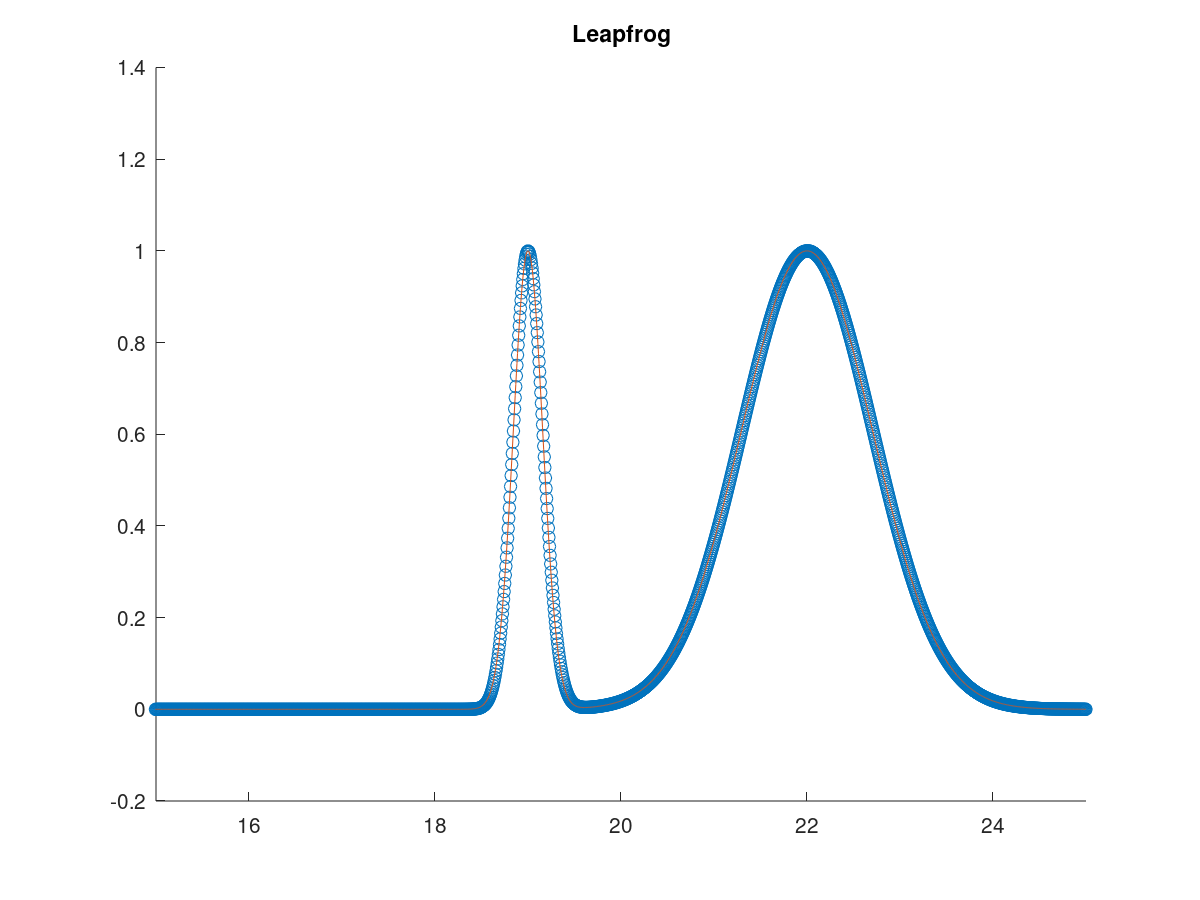
\includegraphics[scale = 0.17]{Leapfrog8.png}
        \end{tabular}
    \label{tbl:table_of_figures}
    \caption{Da esquerda para a direita são $h = 0.05, h = 0.025,h = 0.0125, h = 0.00625$}.
\end{table}

\newpage
\subsection{Lax-Wardroff}
\begin{table}[h]
    \centering
        \begin{tabular}{ccccc}
            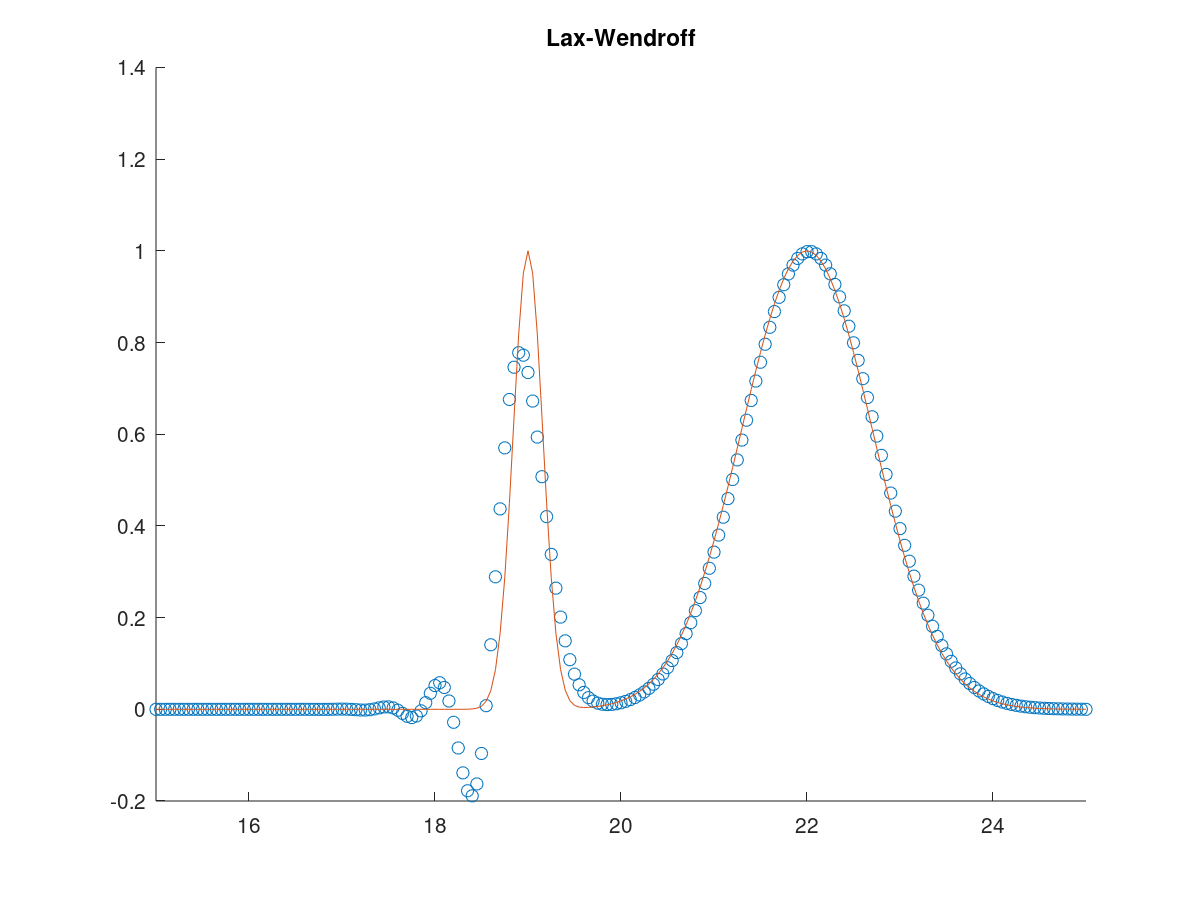
\includegraphics[scale = 0.17]{LW.png} & 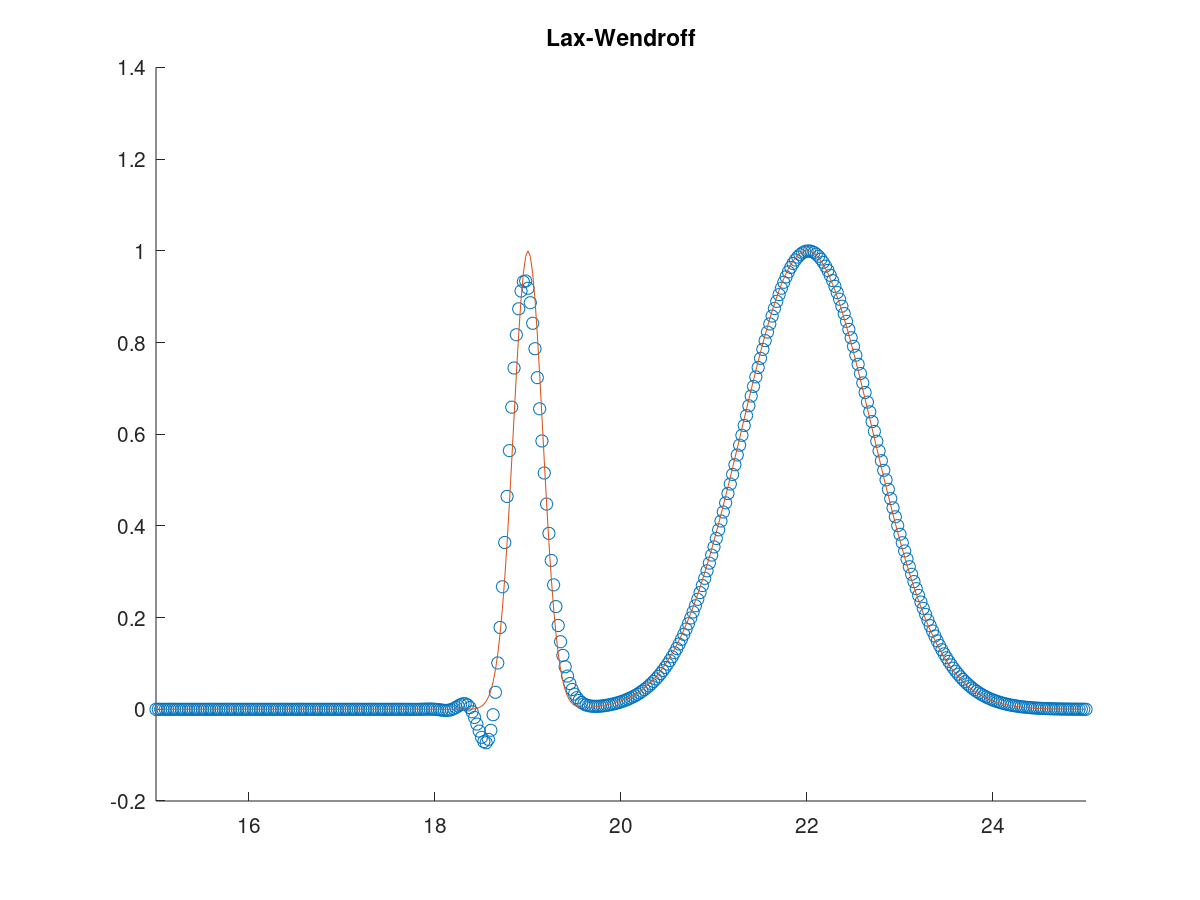
\includegraphics[scale = 0.17]{LW2.png} \\
            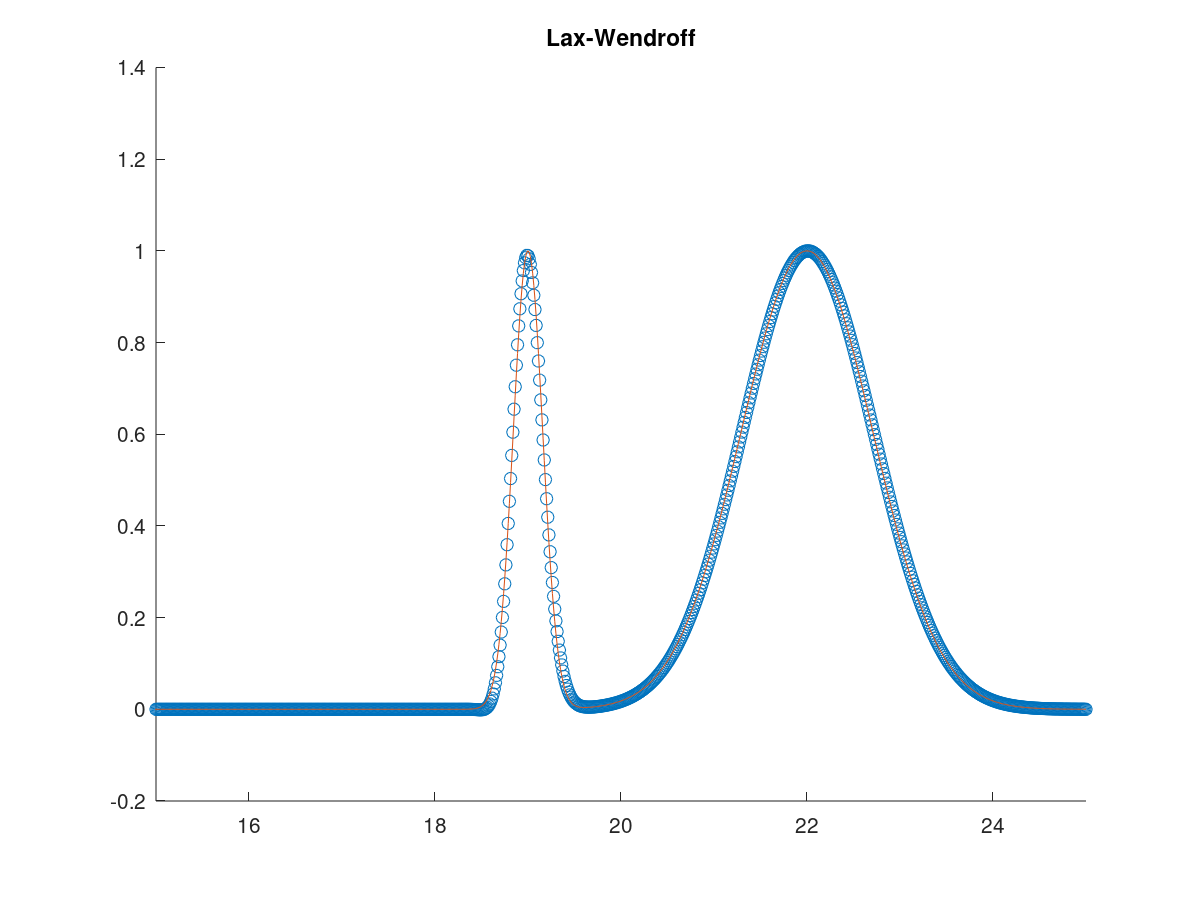
\includegraphics[scale = 0.17]{LW4.png} & 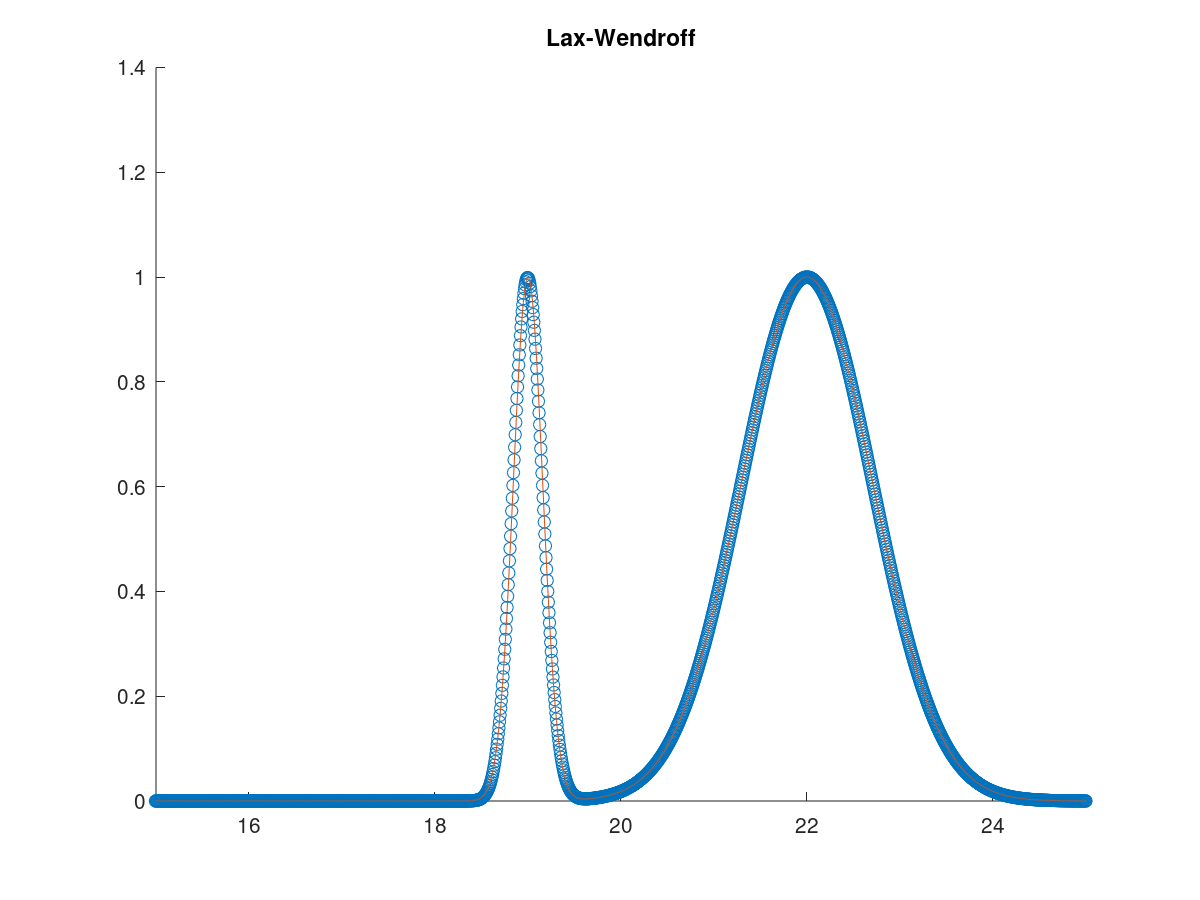
\includegraphics[scale = 0.17]{LW8.png}
        \end{tabular}
    \label{tbl:table_of_figures}
    \caption{Da esquerda para a direita são $h = 0.05, h = 0.025,h = 0.0125, h = 0.00625$}.
\end{table}

\subsection{Conclusão}
É facil ver que \textbf{Lax-Wardroff} e \textbf{Leapfrog} são os melhores métodos. Em especial o método Leapfrog teria o melhor resultado teórico, com $\mathcal{O}(h^4)$, mas nessa discretização em particular obteve um resultado muito similar ao método L-W, de ordem $\mathcal{O}(h^3)$.














\end{document}
